\documentclass[10pt]{article}
\usepackage[T1]{fontenc}
\usepackage{amsmath,amssymb}
\usepackage{graphicx}
\usepackage{booktabs}
\usepackage[margin=1in]{geometry}
\usepackage[hidelinks]{hyperref}

\title{Predictive Warm Pools for Serverless Cold-Start Reduction}
\author{Lin Zhou\\Department of Computer Science}
\date{}

\begin{document}
\maketitle

\begin{abstract}
Serverless platforms start a fresh sandbox whenever a request arrives for a
function that has no idle instance, and this cold start can add hundreds of
milliseconds to the response time. Platforms therefore keep finished instances
warm for a fixed period, which wastes memory on functions that are rarely
called and still misses bursts on functions that are called often. We present
WarmCast, a controller that forecasts the arrival rate of each function and
sizes a pool of pre-started instances to minimise the sum of memory cost and
cold-start cost. On a two-week production trace, WarmCast reduces the
cold-start rate from 18.4\% to 6.1\% while using 22\% less idle memory than a
ten-minute keep-alive policy.
\end{abstract}

\section{Introduction}
\label{sec:intro}

Function-as-a-Service (FaaS) lets developers deploy individual functions and
pay only for the time they run~\cite{jonas2019cloud}. The platform hides
servers, scaling and placement, but it cannot hide the cost of starting a
sandbox. When a request finds no idle instance of its function, the platform
must create a container or microVM, load the language runtime and initialise
the application, which together take between 100\,ms and several
seconds~\cite{wang2018peeking,oakes2018sock}. Such cold starts dominate the
tail latency of short functions.

Most platforms use a simple keep-alive policy: after an instance finishes a
request, it stays in memory for a fixed period, typically ten minutes, in case
another request arrives~\cite{shahrad2020serverless}. This policy is easy to
deploy, but it treats every function the same. A function invoked once per
hour holds memory for ten minutes and is still cold on its next call, while a
function with bursty traffic needs several instances at once and receives
only one.

We observe that the arrival rate of most functions changes slowly compared
with the time needed to start an instance. A short-term forecast of the rate
is therefore enough to decide how many instances to keep ready. Building on
this observation, we make three contributions. First, we model the number of
arrivals in the next interval as a Poisson variable whose rate is estimated
online (Section~\ref{sec:method}). Second, we derive the pool size that
minimises the expected cost of idle memory and cold starts, which has a
closed form for a given rate. Third, we evaluate the resulting controller,
WarmCast, on a production trace and show that it dominates fixed keep-alive
policies on both cost and latency (Section~\ref{sec:eval}).

\section{Related Work}
\label{sec:related}

Prior work reduces cold starts in two ways: by making each start cheaper, or
by starting fewer instances. On the first front, SOCK~\cite{oakes2018sock}
caches imported packages in a zygote process, Firecracker~\cite{agache2020firecracker}
boots a minimal microVM in about 125\,ms, and Catalyzer~\cite{du2020catalyzer}
restores an initialised instance from a checkpoint. SAND~\cite{akkus2018sand}
runs functions of the same application in one container to share their start
cost. These techniques shorten each cold start but do not change how often
one occurs.

On the second front, Shahrad et al.~\cite{shahrad2020serverless} characterise
the Azure Functions workload and propose a hybrid histogram policy that
chooses the keep-alive and pre-warming windows for each application.
FaasCache~\cite{fuerst2021faascache} treats warm instances as a cache and
evicts them with a Greedy-Dual policy. Both approaches decide when to keep a
single instance alive. WarmCast instead decides how many instances to keep,
which matters for functions whose requests arrive in bursts.

Our forecaster is deliberately lightweight. We use exponential
smoothing~\cite{hyndman2021forecasting} because it needs constant memory per
function and adapts within a few intervals; heavier models such as recurrent
networks would cost more to run than the cold starts they avoid for most
functions. Platforms built on OpenLambda~\cite{hendrickson2016openlambda}
expose the per-minute counts that the forecaster needs.

\section{Method}
\label{sec:method}

WarmCast runs as a controller next to the platform scheduler. Time is divided
into intervals of length $\tau$, which we set to one minute. At the start of
each interval the controller updates a rate estimate for every function,
computes a target pool size, and starts or stops pre-warmed instances to
reach it. Requests are routed to warm instances first; a request that finds
none triggers a cold start as before.

\paragraph{Rate estimation.}
Let $x_t$ be the number of requests a function received in interval $t$. We
estimate its arrival rate with exponential smoothing,
\begin{equation}
  \hat{\lambda}_t = \alpha \, \frac{x_t}{\tau} + (1 - \alpha) \, \hat{\lambda}_{t-1},
  \label{eq:ewma}
\end{equation}
where $\alpha \in (0, 1]$ controls how quickly the estimate follows a change
in load. A large $\alpha$ reacts to bursts but also to noise; we use
$\alpha = 0.3$, which performed best on a held-out day of the trace.

\paragraph{Pool sizing.}
Given the rate, we model the number of arrivals $N$ in the next interval as a
Poisson variable with mean $\mu = \hat{\lambda}_t \tau$. If $k$ instances are
warm, every arrival beyond the $k$-th concurrent one causes a cold start. Let
$c_m$ be the cost of keeping one instance in memory for an interval and $c_s$
the cost of one cold start. The expected cost of a pool of size $k$ is
\begin{equation}
  C(k) = c_m \, k + c_s \, \mathbb{E}\big[(N - k)^{+}\big],
  \label{eq:cost}
\end{equation}
and the controller chooses $k^{*} = \arg\min_{k \ge 0} C(k)$. Because $C$ is
convex in $k$, the minimiser is the smallest $k$ for which
$\Pr[N > k] \le c_m / c_s$, which we find by evaluating the Poisson tail from
$k = 0$ upward.

\paragraph{Cost parameters.}
We express both costs in GB-seconds of memory. The memory cost $c_m$ is the
memory size of the function times $\tau$, and the start cost $c_s$ is the
memory size times the measured cold-start duration, multiplied by a weight
$w$ that encodes how much the operator values latency over memory. With
$w = 1$ the controller minimises total memory time; larger values buy lower
latency with more memory.

\paragraph{Safety limits.}
To avoid holding memory for a function whose traffic has stopped, the
controller caps $k^{*}$ at the largest number of concurrent requests observed
in the last hour and releases all instances of a function that received no
request for 30 minutes. Pre-warming uses spare capacity only; when a host
runs short of memory, pre-warmed instances are evicted before instances that
serve requests.


\section{Evaluation}
\label{sec:eval}

We replay the first two weeks of the Azure Functions
trace~\cite{shahrad2020serverless}, which records per-minute invocation
counts, execution times and memory sizes for 46\,413 functions. We use day~1
to tune $\alpha$ and $w$ and report results on days 2--14. Cold-start
durations are drawn from the per-runtime distribution measured by Wang et
al.~\cite{wang2018peeking}.
% TODO: report variance over random seeds

We compare WarmCast with three policies: a fixed keep-alive of 10 minutes
(\emph{KA-10}), the same policy with a 60-minute window (\emph{KA-60}), and
the hybrid histogram policy of Shahrad et al.\ (\emph{Hybrid}). All policies
run on the same simulated cluster of 200 hosts with 64\,GB of memory each.

Our simulator is event-driven and models the memory of each host but not its
CPU. It assumes that a warm instance serves a request immediately and that a
cold start blocks the request for the full start duration. These assumptions
favour no policy in particular, since all policies share them.

\begin{table}[t]
  \centering
  \caption{Results on days 2--14 of the trace. Idle memory is the average
    memory held by idle instances.}
  \label{tab:main}
  \begin{tabular}{lrrr}
    \toprule
    Policy   & Cold starts (\%) & P99 latency (ms) & Idle memory (TB) \\
    \midrule
    KA-10    & 18.4 & 1240 & 2.31 \\
    KA-60    &  6.8 &  410 & 7.02 \\
    Hybrid   &  9.7 &  655 & 2.05 \\
    WarmCast &  6.1 &  388 & 1.80 \\
    \bottomrule
  \end{tabular}
\end{table}

Table~\ref{tab:main} summarises the results. WarmCast lowers the cold-start
rate to 6.1\%, compared with 18.4\% for KA-10 and 9.7\% for Hybrid, while
holding less idle memory than either. KA-60 reaches a similar cold-start rate
only by keeping almost four times as much memory idle. The 99th-percentile
latency follows the cold-start rate, since most requests in the tail are
cold.

\begin{figure}[t]
  \centering
  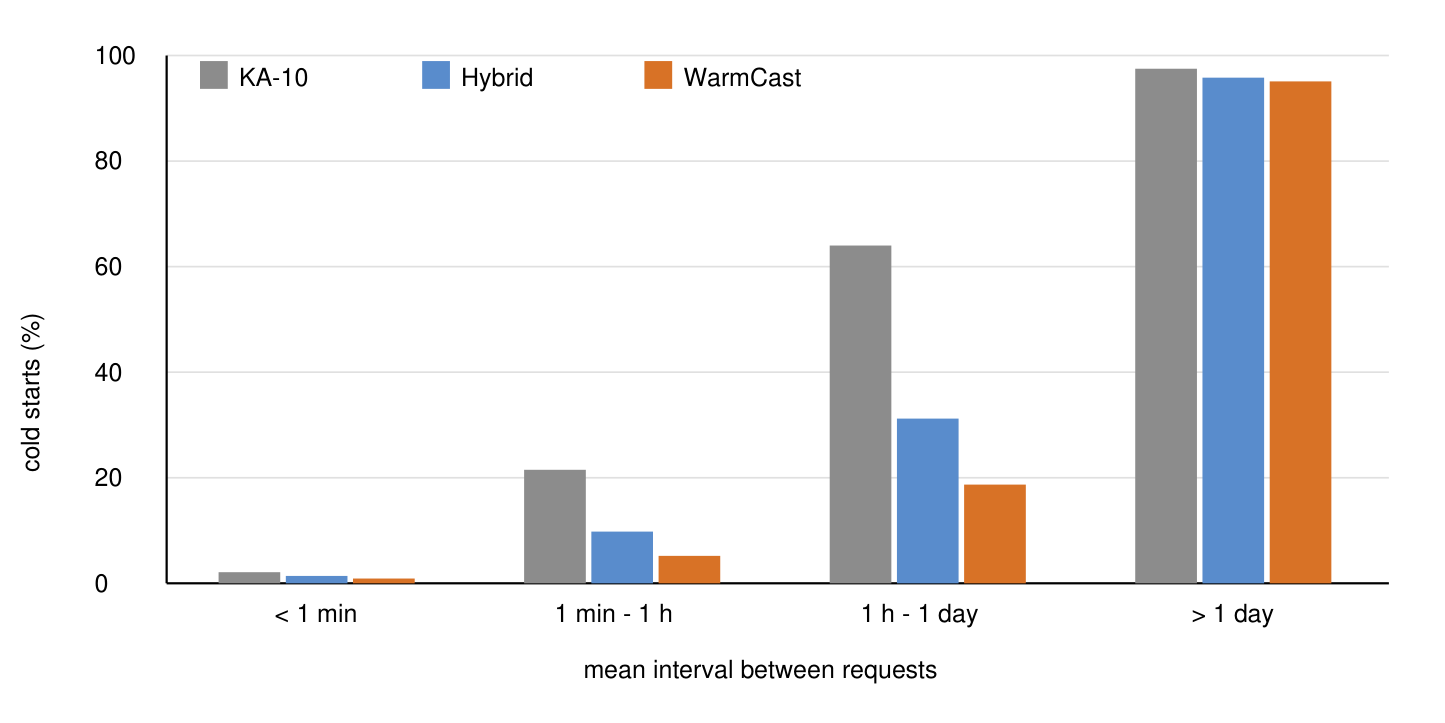
\includegraphics[width=0.8\linewidth]{figures/coldstart.png}
  \caption{Cold-start rate by invocation frequency. Each group of bars covers
    the functions whose mean interval between requests falls in the given
    range.}
  \label{fig:coldstart}
\end{figure}

Figure~\ref{fig:coldstart} breaks the cold-start rate down by how often a
function is invoked. Rarely invoked functions are cold under every policy,
because no forecast can predict a single request per day. The gain of
WarmCast comes from functions invoked between once per minute and once per
hour, where fixed windows either expire too early or hold instances for too
long.

The controller adds little overhead. Updating the estimate in
Eq.~\eqref{eq:ewma} and searching for $k^{*}$ take 3.2\,$\mu$s per function
on one core, so a single controller thread handles all 46\,413 functions
within 0.2\,s per interval. The memory footprint is two floating-point numbers
per function. We did not observe any measurable effect of the controller on
request latency in a prototype deployment.

\section{Conclusion}
\label{sec:conclusion}

We presented WarmCast, which sizes a pool of warm instances for each
serverless function from a short-term forecast of its arrival rate. The pool
size follows from a convex cost model with a closed-form minimiser, and the
controller runs in microseconds per function. On a production trace it
reduces cold starts by a factor of three compared with the default keep-alive
policy while holding less idle memory. In future work we plan to share warm
instances between functions with the same runtime and to forecast with
seasonal models.

\begin{thebibliography}{10}

\bibitem{agache2020firecracker}
A.~Agache, M.~Brooker, A.~Iordache, A.~Liguori, R.~Neugebauer, P.~Piwonka,
  and D.-M. Popa.
\newblock Firecracker: Lightweight virtualization for serverless applications.
\newblock In \emph{Proc.\ USENIX NSDI}, pages 419--434, 2020.

\bibitem{akkus2018sand}
I.~E. Akkus, R.~Chen, I.~Rimac, M.~Stein, K.~Satzke, A.~Beck, P.~Aditya, and
  V.~Hilt.
\newblock {SAND}: Towards high-performance serverless computing.
\newblock In \emph{Proc.\ USENIX ATC}, pages 923--935, 2018.

\bibitem{du2020catalyzer}
D.~Du, T.~Yu, Y.~Xia, B.~Zang, G.~Yan, C.~Qin, Q.~Wu, and H.~Chen.
\newblock Catalyzer: Sub-millisecond startup for serverless computing with
  initialization-less booting.
\newblock In \emph{Proc.\ ASPLOS}, pages 467--481, 2020.

\bibitem{fuerst2021faascache}
A.~Fuerst and P.~Sharma.
\newblock {FaasCache}: Keeping serverless computing alive with greedy-dual
  caching.
\newblock In \emph{Proc.\ ASPLOS}, pages 386--400, 2021.

\bibitem{hendrickson2016openlambda}
S.~Hendrickson, S.~Sturdevant, T.~Harter, V.~Venkataramani, A.~C.
  Arpaci-Dusseau, and R.~H. Arpaci-Dusseau.
\newblock Serverless computation with {OpenLambda}.
\newblock In \emph{Proc.\ USENIX HotCloud}, 2016.

\bibitem{hyndman2021forecasting}
R.~J. Hyndman and G.~Athanasopoulos.
\newblock \emph{Forecasting: Principles and Practice}.
\newblock OTexts, 3rd edition, 2021.

\bibitem{jonas2019cloud}
E.~Jonas, J.~Schleier-Smith, V.~Sreekanti, C.-C. Tsai, A.~Khandelwal, Q.~Pu,
  V.~Shankar, J.~Carreira, K.~Krauth, N.~Yadwadkar, J.~E. Gonzalez, R.~A.
  Popa, I.~Stoica, and D.~A. Patterson.
\newblock Cloud programming simplified: A {Berkeley} view on serverless
  computing.
\newblock Technical Report UCB/EECS-2019-3, UC Berkeley, 2019.

\bibitem{oakes2018sock}
E.~Oakes, L.~Yang, D.~Zhou, K.~Houck, T.~Harter, A.~Arpaci-Dusseau, and
  R.~Arpaci-Dusseau.
\newblock {SOCK}: Rapid task provisioning with serverless-optimized
  containers.
\newblock In \emph{Proc.\ USENIX ATC}, pages 57--70, 2018.

\bibitem{shahrad2020serverless}
M.~Shahrad, R.~Fonseca, I.~Goiri, G.~Chaudhry, P.~Batum, J.~Cooke,
  E.~Laureano, C.~Tresness, M.~Russinovich, and R.~Bianchini.
\newblock Serverless in the wild: Characterizing and optimizing the serverless
  workload at a large cloud provider.
\newblock In \emph{Proc.\ USENIX ATC}, pages 205--218, 2020.

\bibitem{wang2018peeking}
L.~Wang, M.~Li, Y.~Zhang, T.~Ristenpart, and M.~Swift.
\newblock Peeking behind the curtains of serverless platforms.
\newblock In \emph{Proc.\ USENIX ATC}, pages 133--146, 2018.

\end{thebibliography}

\end{document}
